\documentclass[11pt]{article}
\usepackage[T1]{fontenc}
\usepackage[utf8]{inputenc}
\usepackage[portuguese]{babel}
\usepackage{amsmath}
\usepackage{graphicx}
\usepackage{float}
\usepackage{enumitem}

\graphicspath{{}}

\newcommand{\numpy}{{\tt numpy}}

\topmargin -.5in
\textheight 9in
\oddsidemargin -.25in
\evensidemargin -.25in
\textwidth 7in

\begin{document}

    \author{Lucas Emanuel Resck Domingues}
    \title{Aula prática 5
    \medbreak
    \large Decomposição QR}
    \maketitle
    
    \medskip
    
    \begin{enumerate}
    
        \item %1
        
            A função Scilab \textbf{gram\_schmidt} foi escrita no arquivo \textbf{Functions.sce}. Vejamos como ela se comporta para as seguintes matrizes:
        
            \begin{figure}[H]
                \centering
                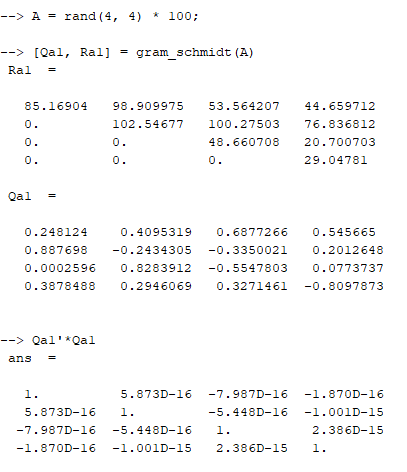
\includegraphics[]{1-1}
                \caption{Matriz $A_{4\times4}$ e método de Gram-Schmidt.}
            \end{figure}
        
            Para essa matriz $4\times4$, a função encontra uma matriz $R$ triangular superior. Além disso, dado que buscamos $Q$ tal que $Q^TQ = I$ , temos que $Q^TQ \approx I$, ou seja, isso indica uma boa precisão do método.
        
            \begin{figure}[H]
                \centering
                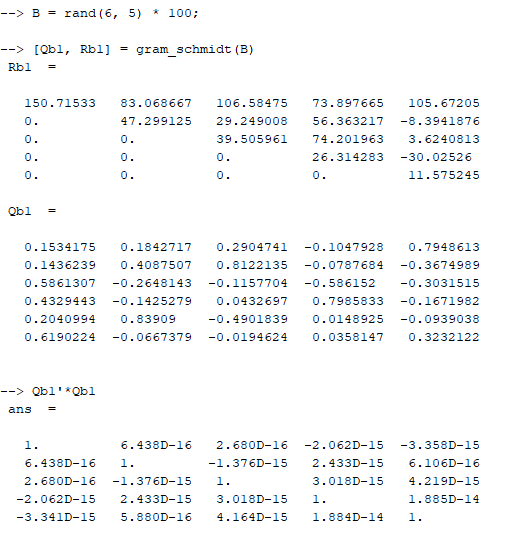
\includegraphics[]{1-2}
                \caption{Matriz $A_{6\times5}$ e método de Gram-Schmidt.}
            \end{figure}
            
            Para essa matriz $6\times5$, obtemos uma $R$ triangular superior. Além disso, $Q^TQ \approx I$ indica uma boa precisão do método.
            
            Concluímos que a função \textbf{gram\_schmidt} cumpre o esperado.
        
        \bigbreak
        
        \item %2
        
            A função Scilab \textbf{gram\_schmidt\_modificado} foi escrita no arquivo \textbf{Functions.sce}. Vejamos como ela se comporta para as mesmas matrizes do item anterior.
        
            \begin{figure}[H]
                \centering
                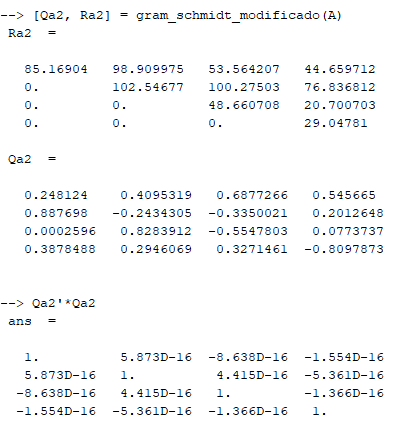
\includegraphics[]{2-1}
                \caption{Matriz $A_{4\times4}$ e método de Gram-Schmidt modificado.}
            \end{figure}
        
            A função encontra uma matriz $R$ triangular superior e temos que $Q^TQ \approx I$, ou seja, o método tem boa aproximação. Comparando a precisão desse método com o do item anterior:
        
            \begin{figure}[H]
                \centering
                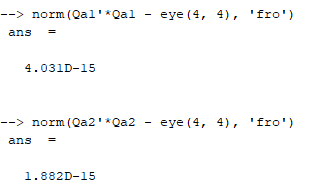
\includegraphics[]{2-2}
                \caption{Comparação da precisão entre os métodos de Gram-Schmidt e Gram-Schmidit modificado utilizando a norma de Frobenius.}
            \end{figure}
            
            Foi utilizada a norma de Frobenius na matriz $Q^TQ - I$ para o cálculo da precisão do método. Uma matriz ideal teria norma $0$. Observe que o método de Gram-Schmidt modificado obteve uma melhor precisão para essa matriz.
        
            \begin{figure}[H]
                \centering
                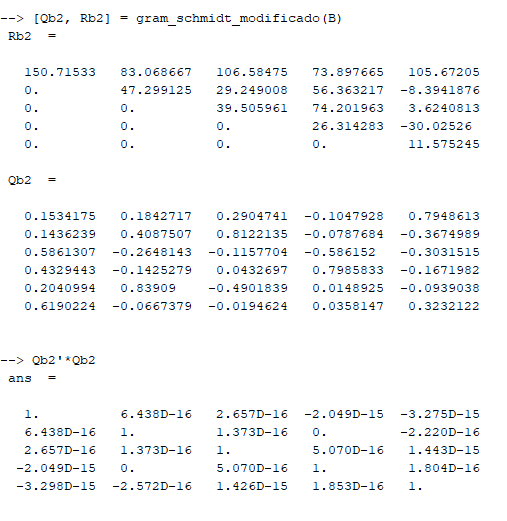
\includegraphics[]{2-3}
                \caption{Matriz $A_{6\times5}$ e método de Gram-Schmidt modificado.}
            \end{figure}
        
            A função encontra uma matriz $R$ triangular superior e temos que $Q^TQ \approx I$. Comparando a precisão desse método com o do item anterior:
        
            \begin{figure}[H]
                \centering
                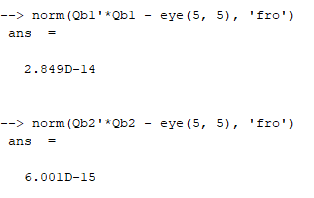
\includegraphics[]{2-4}
                \caption{Comparação da precisão entre os métodos de Gram-Schmidt e Gram-Schmidit modificado utilizando a norma de Frobenius.}
            \end{figure}
            
            O cálculo da precisão do método é análogo ao anterior. Observe que o método de Gram-Schmidt modificado obteve uma melhor precisão para essa matriz.
            
            Concluímos que a função \textbf{gram\_schmidt\_modificado} cumpre o esperado e tem melhor precisão do que a função \textbf{gram\_schmidt}.
        
        \bigbreak
        
        \item %3
        
            A função Scilab \textbf{householder} foi escrita no arquivo \textbf{Functions.sce}. Vejamos como ela se comporta para as mesmas matrizes do item anterior.
        
            \begin{figure}[H]
                \centering
                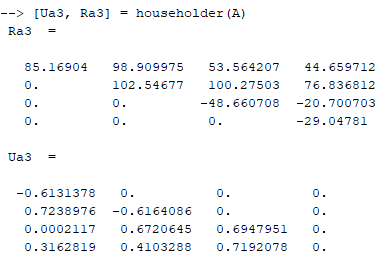
\includegraphics[]{3-1}
                \caption{Matriz $A_{4\times4}$ e método de Householder.}
            \end{figure}
        
            A função encontra uma matriz $R$ triangular superior e nos retorna uma matriz $U$ com os vetores unitários que geram as matrizes de Householder. Comparando a precisão desse método com a dos itens anteriores:
        
            \begin{figure}[H]
                \centering
                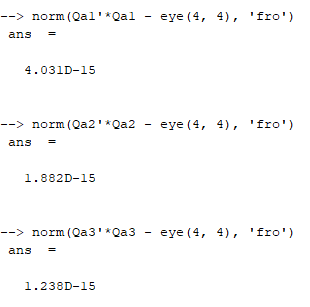
\includegraphics[]{3-2}
                \caption{Comparação da precisão entre os métodos utilizando a norma de Frobenius.}
            \end{figure}
            
            É possível calcular $Q$ a partir da matriz $U$ e isso foi feito. O cálculo da precisão do método é feito da mesma forma que anteriormente. Observe que o método de Householder tem melhor precisão para essa matriz.
        
            \begin{figure}[H]
                \centering
                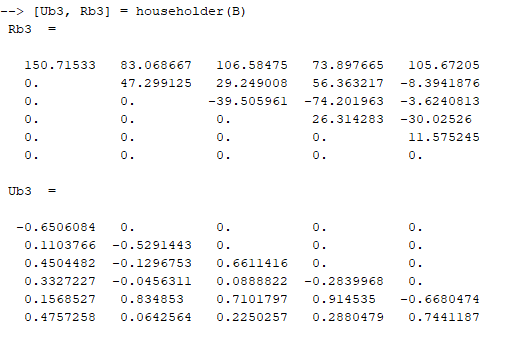
\includegraphics[]{3-3}
                \caption{Matriz $A_{6\times5}$ e método de Householder.}
            \end{figure}
        
            A função retorna as matrizes $R$ e $U$ que esperamos. Comparando a precisão desse método com as dos itens anteriores:
        
            \begin{figure}[H]
                \centering
                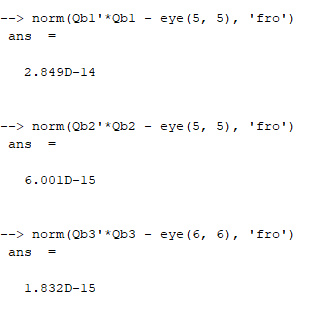
\includegraphics[]{3-4}
                \caption{Comparação da precisão entre os métodos utilizando a norma de Frobenius.}
            \end{figure}
            
            O cálculo da precisão do método é análogo ao anterior. Observe que o método de Householder teve melhor precisão para esta matriz.
            
            Concluímos que a função \textbf{householder} cumpre o esperado e tem melhor precisão do que as funções \textbf{gram\_schmidt} e \textbf{gram\_schmidt\_modificado}.
        
        \bigbreak
        
        \item %4
        
            \begin{enumerate}[label=\arabic*)]
                \setcounter{enumii}{1}
                \item %2
                
                \begin{enumerate}[label=\alph*)]
                    \item Queremos aproximar $s(t) = s_0 + v_0t + \frac{1}{2}gt^2$. Formemos $A$ e $b$:
                
                    $$A = \begin{bmatrix}
                    1& 0,5& 0,25\\
                    1& 1& 1\\
                    1& 1,5& 2,25\\
                    1& 2& 4\\
                    1& 3& 9
                    \end{bmatrix}\textrm{, }
                    b = \begin{bmatrix}
                    11\\
                    17\\
                    21\\
                    23\\
                    18
                    \end{bmatrix}$$
                    
                    Precisamos encontrar $\mathbf{x}$ tal que $A^TA\mathbf{x}=A^Tb$. Porém, agora, podemos encontrá-lo fatorando $A$ em $Q$ e $R$ e resolvendo $R\mathbf{x} = Q^Tb$. Utilizando a função \textbf{gram\_schmidt\_modificado} para a fatoração QR e a função \textbf{Gaussian\_Elimination\_4}, da aula prática 1, para a resolução do sistema:
        
                    \begin{figure}[H]
                        \centering
                        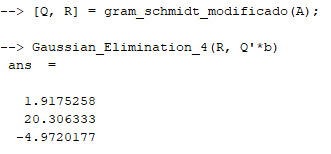
\includegraphics[]{4-1}
                        \caption{Fatoração QR e resolução do sistema.}
                    \end{figure}
                    
                    Então obtemos $\mathbf{x} = (s_0, v_0, \frac{g}{2}) \approx (1,92; 20,31; -4,97)$.
                    
                    Os resultados foram muito próximos daqueles obtidos na aula prática 4, então, neste caso, não seria necessária a fatoração QR através do método de Gram-Schmidt modificado.
                    
                    \bigbreak
                    
                    \item $s_0 \approx 1,92 \textrm{m}$, $v_0 \approx 20,31\textrm{m/s}$ e $g \approx -9,94 \textrm{m/s}^2$.
                    
                    \bigbreak
                    
                    \item Resolvendo $0 = s_0 + v_0t + \frac{1}{2}gt^2$, obtemos $t\approx 4,18 \textrm{s}$.
                    
                \bigbreak
                \end{enumerate}
                
                \item
                
                \begin{enumerate}[label=\alph*)]
                    \item Vamos aproximar $y = p(t) = ce^{kt}$. Podemos aproximar $\ln y = \ln c + kt$, um modelo linear, então $\mathbf{x} = (\ln c, k)$. Calculamos $b$ aplicando $\ln$ nas populações. Realizamos a fatoração QR da matriz $A$ utilizando a função \textbf{householder}, encontramos a matriz $Q$ a partir da matriz $U$ e, com a função \textbf{Gaussian\_Elimination\_4}, da aula prática 1, resolvemos $R^TR\mathbf{x} = R^TQ^Tb$. Considerando $t=0$ para $1950$, temos:
                
                    \begin{figure}[H]
                        \centering
                        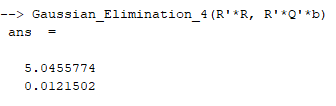
\includegraphics[]{4-2}
                        \caption{Resolução do sistema $R^TR\mathbf{x} = R^TQ^Tb$.}
                    \end{figure}
                    
                    Calculamos a solução de $R^TR\mathbf{x} = R^TQ^Tb$ pois $R^T$ não é invertível.
                    
                    Novamente, os resultados foram muito próximos daqueles obtidos na aula prática 4. Sendo assim, a fatoração QR pelo método de Householder não é muito necessária neste caso.
                    
                    Concluímos que $c \approx e^{5,04} \approx 155,33$ e $k \approx 0,01$. Logo, $p(t)\approx155,33e^{0,01t}$. Portanto, a taxa de crescimento é $p'(t) \approx 1,89e^{0,01t}$.
                    \bigbreak
                    \item A população estimada dos EUA em 2010 é $p(60) = ce^{k60} \approx 322,01$ milhões de pessoas. Em 2010, a população dos EUA foi de $309,3$ milhões de pessoas. Nosso modelo superestimou a população. Sabemos que um modelo exponencial não se adequa muito bem a um crescimento populacional de uma população já grande.
                    \bigbreak
                    
                \end{enumerate}
                
            \end{enumerate}
        
        
    \end{enumerate}
\end{document}
\grid
\grid